\scanpage{92}
et les isom de transitivité de $1^\circ$ \unsure{\ldots}

$-$

$4^\circ)$ Formules de changt de base (auraient intérêt \unsure{à être|: être} bloquées après $1^\circ$)

\diagram{\begin{tikzcd}[ampersand replacement=\&]
X \& X' \arrow[l,"g'"']\\
Y \& Y' \arrow[l,"g"] \arrow[u,phantom]
\arrow[from=1-1,to=2-1,"f"'] \arrow[from=1-2,to=2-2,"f'"]
\end{tikzcd}}

\[
\boxed{\boxed{\mathbb{L}g^*\mathbb{R}_!f_*\xrightarrow{\sim}\mathbb{R}_!f'_*\mathbb{L}g'^*}}
\]
\margin{ch. de base pour morphismes \uline{propres}}
\margin{\figure{
\begin{tikzpicture}
\draw (0,0)--(1,1.5);
\draw (0,0)--(1,.3);
\draw (0,0)--(.7,-.6);
\node[align=left] at (-.4,-.6) {\unsure{à priori quelle}\\\unsure{?}};
\end{tikzpicture}}}
\[
\left\{
\begin{aligned}
\mathbb{L} g^{\deleted{\unsure{*}}*}\mathbb{R}f_*&\xrightarrow{\sim}\mathbb{R}f'_*\mathbb{L}g'^*
&&\text{si $f$ propre \boxed{\text{ou $g$ lisse}}}\\
\uuline{\mathbb{R}^{\inserted{!}}f^{\deleted{\unsure{*}}\inserted{'}}\mathbb{L}g^*}
&\uuline{\xleftarrow{\sim}\deleted{\unsure{\mathbb{R}^*}}\inserted{\mathbb{L}}g'^*\mathbb{R}^{\inserted{!}}f^{\deleted{\unsure{*}}}}
&&\text{si $f$ ou \boxed{\text{$g$ lisse}}}
\end{aligned}
\right.
\]
\figure{\begin{tikzpicture}
\node (a) at (0,0) {$\boxed{\mathbb{R}^!g\mathbb{R}_!^{\deleted{\unsure{*}}}f\xrightarrow{\sim}\mathbb{R}_!^{\deleted{\unsure{*}}}f'\mathbb{R}^!g'}$};
\draw[decorate,decoration={snake,amplitude=1pt,segment length=12pt}] (-3.0,-.4) rectangle (3.0,.4);
\node at (5.0,0) {si $f$ propre ou $g$ lisse};
\node[draw,double] (b) at (0,-1.2) {$\mathbb{R}^!g\mathbb{R}f_*\simeq \mathbb{R}f'_*\mathbb{R}^!g'$};
\draw[<->] (-3.6,.4) -- (-3.6,-1.5);
\node[rotate=22] at (-4.0,.5) {$g$ lissifiable};
\node[align=left] (c) at (7,-1.1) {$\Leftrightarrow$ (\unsure{se décompose en cas lisse}\\
$={}$ changt de base lisse, et cas d'une\\
immersion, trivial)};
\node[align=left] (d) at (6.7,1.2) {changt de\\base lisse};
\draw[<->] (6.7,1.7) -- (6.7,2.3);
\draw[->] (d.east) to[bend left=35] (c.north east);
\node (e) at (1,-2.5) {est une conséquence du précédent};
\draw[->] (-3.2,.5) to[bend right=30] (e.west);
\end{tikzpicture}}

$5^\circ)$ \uline{Formules d'induction}
\[
\boxed{\mathbb{R}^!f(\mathbb{R}\operatorname{Hom}(F^\bullet,G^\bullet))
\simeq \mathbb{R}\operatorname{Hom}(\mathbb{L}f^*(F^\bullet),\mathbb{R}^!f(G^\bullet))}
\]
\diagram{\begin{tikzcd}[ampersand replacement=\&]
X\arrow[d,"f"]\\
Y\quad F,G
\end{tikzcd}}
\[
\boxed{\mathbb{L}f^*(F^\bullet\mathbin{\overset{\mathbb{L}}{\otimes}}G^\bullet)
\simeq \mathbb{L}f^*(F^\bullet)\mathbin{\overset{\mathbb{L}}{\otimes}}\mathbb{L}f^*(G^\bullet)}
\]
\margin{formule pour topos annelés quelconques \unsure{\ldots}}
\mspage{91}
